\section{Case study: NASA's forest fire API}\label{sec:attack}

\begin{figure}
  \centering
  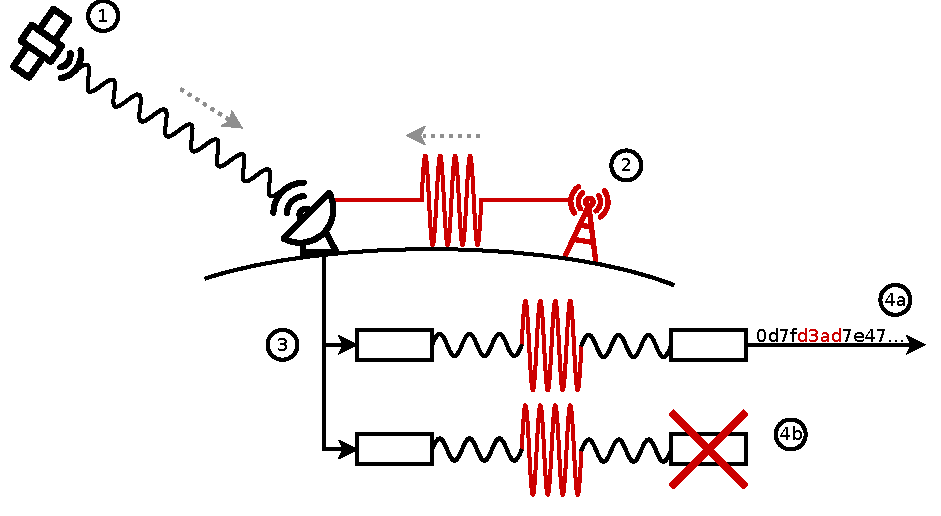
\includegraphics[width=\columnwidth]{diagrams/attack_illustration.pdf}
  \caption{An illustration of the attacks described in this paper. The attacker is indicated in red. 1)~The satellite broadcasts a signal; 2)~A ground-based attacker injects a crafted signal, overshadowing the legitimate signal and resulting in one of two scenarios; 3a)~The victim receiver decodes the attacker-controlled data, poisoning derived datasets; 3b)~The injected signal exploits vulnerabilities in the protocol decoders, resulting in denial of service or arbitrary code execution.}
  \label{fig:attack-illustration}
\end{figure}

% An end-to-end case study of how an attacker could target NASA's real time forest fire API

In this section we explore an end-to-end case study of overshadowing attacks against the \textit{Fire Information and Resource Management System} (FIRMS), NASA's real time forest fire API.
We begin with a discussion of its architecture, focusing on the SATCOM link.
Using only publicly documented information, we write a packet encoder for the protocol, and set up the decoding software as used by NASA in a test environment.

We explore poisoning the derived datasets by injecting ficticious images, and exploitation of processing stages by injecting malformed data, using the data derived from overshadowing our generated signal on top of a legitimate signal.

% We calculate the overshadow ratio...

\subsection{Mission architecture}

FIRMs is a NASA project, which provides a worldwide map of active forest fires, each with precise coordinates and a confidence value.
A real-time fire notification service is provided which is used for emergency response, disaster planning, and crisis analysis, and is sent to users in more than 160 countries~\cite{firmsUsage}.
The data is derived from several satellites in the Earth Observing System (EOS) fleet.

\subsubsection{Earth observing satellites}

Specifically,\textit{Terra}, \textit{Aqua}, and \textbf{TODO} are the EOS fleet satellites whose data is used for FIRMS.
They are equipped with sensors such as MODIS~\footnote{Moderate Resolution Imaging Spectroradiometer} which provide calibrated light readings across frequency bands wider than the visible spectrum.
The presence of a fire is derived primarily from the infrared bands~\cite{mod14Manual}, which can reveal hotspots on the surface.
MODIS datasets are also used for a number of other research purposes, including recently to analyze weather-dispersed diseases that pose serious risks to human health~\cite{valleyFever}.

Thanks to their opposite polar sun-synchronous orbits, Terra and Aqua together image the entire surface of the Earth each day.
The data is then downlinked by one of two mechanisms -- either as a continuous stream known as \textit{direct broadcast}, or via a data dump through TDRSS, NASA's relay satellites.
The data is unencrypted by design, since these satellites were intended to have public data.
The community is therefore encouraged to set up custom receiver stations.
As a result, MODIS data is widely available both from the central NASA archives~\cite{ladsweb} and from any of the 168 alternative receiver stations~\cite{nasaDirect}.

\subsubsection{Protocol description}

Terra and Aqua downlink data using the custom \textit{Channel Access Data Unit} (CADU) data link protocol, shown in Figure~\ref{fig:cadu_diagram}.
The CADU is optionally Viterbi encoded (XORed with a fixed polynomial) to prevent desynchronisation during long runs of the same symbol.

The data within each CADU frame is multiplexed from each of the onboard instruments, and is formatted in the highly standard CCSDS \textit{Space Packet Protocol} (SPP), the dominant network layer protocol for space and satellite systems~\cite{modisDescription},p177.
The format is extended with a custom header containing a satellite ID and instrument ID.
The contents of the packet is the raw sensor data; a densely packed array of 12-bit words within the data zone, with a trailing checksum.
Each value represents the intensity of light incident to the sensor of a specific frequency band, which is indicated by the position of the word within the array~\cite{modisDescription},p183-189.

\subsubsection{Decoding software stack}

The data is processed into satellite-derived datasets through NASA's \textit{International Planetary Observation Processing Package}, a software distribution for decoding and processing Earth Observing Systems data.
The software in IPOPP contains protocol decoding stages alongside the satellite-derived dataset generation algorithms.
In particular, the \textit{MODIS Level-1 Science Processing Algorithm} (MODISL1DB\_SPA) is responsible for decoding SPP packets with the MODIS secondary header into the \textit{Heirarchical Data Format} (HDF)~\cite{modisL1DB}.

% These stages are sometimes implemented by dedicated hardware or as a separate piece of software, such as Dartcom's \textit{Polar Orbital Ingester}~\cite{dartcomsystemsltdXBand2021,dartcomPOI}.
% However, they can equivalently be handled by NASA's \textit{Real-time Software Telemetry Processing System} (RT-STPS).

FIRMS derives its dataset from the \textit{MODIS Active Fire Product Science Processing Algorithm} (MOD14\_SPA), which primarily uses the bands of 4 and 11 micrometer wavelengths in the infrared spectrum to detect hotspots.
Therefore, in order to manipulate the detected fires whilst leaving the visible images untouched, the attacker only needs to affect the values in these channels and recalculate the checksum.
This data is geolocated against a terrain map of the Earth, and is ultimately used to generate a CSV of the locations of fires, alongside their intensity and probability.

\textbf{TODO: rest of this subsubsection hasn't been reviewed}

The Level 0 data passes through two stages of the \textit{MODIS Level-1 Science Processing Algorithm} (MODISL1DB\_SPA), resulting in heirarchical data format (HDF) files geolocated to a subpixel accuracy.

The first stage, known as \texttt{l0tol1}, processes Level 0 SPP data into Level 1 HDFs, which contains restructured raw sensor samples alongside other metadata.
The second stage, known as \texttt{l1atob}, geolocates the HDFs to a subpixel accuracy using timing information from the data, the satellite's orbital parameters, and an accurate model of the Earth's surface.
The resulting data is considered to be at Level 1B.

Each of these stages relies upon \textit{OceanColor Science Software} (OCSSW)~\cite{ocssw}, written by the OceanColor Data team \textbf{TODO: check}, to perform the actual processing.
In particular, \textbf{TODO: list the tools for each stage} perform the tasks of extracting the data, and correcting corrupted data in the case of failure.
The OCSSW tools are written in C and Fortran, and were originally designed to be run as command line scripts.
They expect a parameter file at a particular relative path \textbf{TODO: check} which itself describes the location of the data to be processed and supplies options for processing it.

In order to automate processing and correcting the data, Python programs were written which construct the command line arguments and parameter files required for the OCSSW tools, and then invoke a shell to execute the tools.
These are designed to be higher-level tools for use in analysing and processing the data files on the command line, which don't require knowledge of the arcane OCSSW formats.

Within IPOPP, \texttt{l0tol1} and \texttt{l1atob} are themselves shell scripts which call these Python programs with certain arguments callable from the XML interface.
\textbf{TODO: fact check that l1atob is actually a shell script and not the Python directly}

% TODO: link to and cite the software manuals and SPA descriptions of each of these
The geolocated Level 1B HDFs proceed into the next processing stage, the \textit{Level 2 MODIS Active Fire Product} (MOD14).
MOD14 identifies active fires from the MODIS data and outputs HDF and txt files considered to be at Level 2. \textbf{TODO: cite manual}

A summary of the entire pipeline can be found in Figure~\ref{fig:attack_types}.

\begin{figure*}
    \centering
    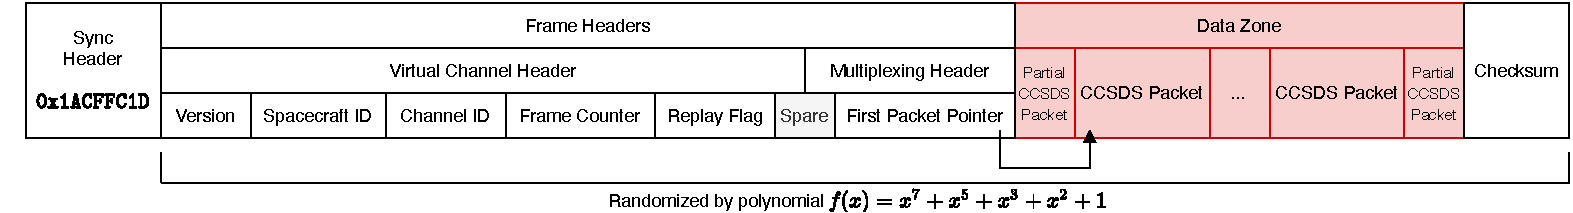
\includegraphics[width=\textwidth]{diagrams/cadu_diagram.pdf}
    \caption{Layout of data within a Channel Access Data Unit (CADU). The section marked in red can contain arbitrary attacker-specified data.}
    \label{fig:cadu_diagram}
\end{figure*}

\subsubsection{Terra and Aqua wireless communications specifications} % TODO: different title?

\textbf{TODO: review this}

% In each of their downlink modes, \textit{Terra} and \textit{Aqua} communicate using frames modulated onto a carrier wave using quadrature phase shift keying (QPSK).
%In QPSK each symbol (pair of bits) is encoded by shifting the phase of the carrier wave
%In QPSK, symbols represent pairs of bits, and are encoded by shifting the phase of the carrier wave in one of four orientati.

%The finalized CADUs are transferred directly to the X-band antenna when in direct broadcast mode, and also to a solid state recorder for playback during the data dumps.
% NB: in the case of EOS, we think the only real difference between the downlinks DB and TDRSS is bit rate, from the space shuttle report

Terra and Aqua communicate on a number of different radio channels and downlink housekeeping, telemetry, and scientific data. \textbf{Are these all the unique ones?}
The satellites themselves can be in one of a number of operational modes, during which they send different information through the available channels. \textbf{TODO: cite SPACE GROUND AQUA document} % TODO: maybe talk about how you can find out more information about this in the appendix?
During nominal operation the satellite is in Direct Broadcast mode, in which the current MODIS sensor data is continuously downlinked.
The data is also buffered for high data rate downlink when the satellite passes over Polar Ground Stations or near its TDRSS relay.

Since the buffer is packed with the same bytes as the Direct Broadcast signal, the format of the data is identical for all modes of broadcast.
We therefore focus on the Direct Broadcast mode without loss of generality.

%To broadcast to the Polar Ground Stations therefore requires a temporary shift out of Direct Broadcast Mode.
%The schedule for direct broadcast can be found for Terra~\cite{terraSchedule} and Aqua~\cite{aquaSchedule} at the HTTP file archive for the Goddard Space Flight Center.

% TODO: describe the structure of each CADU and how the relevant fields e.g. IDs are used
Since each instrument onboard the satellite needs to downlink data simultaneously, the scientific data is sent in a packets to the Formatter/Multiplexer Unit (FMU).
The FMU encapsulates the instrument packets within CCSDS Space Packet Protocol (SPP) packets which contain an Application ID to support demultiplexing per instrument.
The SPP packets are then packed into a custom, unencrypted data link protocol known as the \textit{Channel Access Data Unit}, or CADU.
Finally, the CADUs are modulated onto a radio wave either immediately in the case of Direct Broadcast, or after a short delay for bulk transmission.

The Level 0 data is processed through a pipeline of programs within the IPOPP distribution into subsequently higher levels, eventually resulting in the satellite-derived datasets described in \textbf{TODO: make this table of MODIS data usage}.

\subsection{Generating ficticious data}

To successfully inject forest fires, an attacker needs to manipulate the infrared channels of MODIS packets within the downlinked data.
This data can either be obtained from distributed digital archive centers~\cite{ladsweb} beforehand, or in real time with access to a satellite dish.

Then a decoder can be written

% TODO: write about the process

\subsubsection{Protocol documentation}

\subsubsection{Building the reencoder}

Since existing implementations of the EOS protocols are intended for decoding only, we firstly implement libraries to reencode the data.
We build upon these to demonstrate our attacks end-to-end on the FIRMS software, resulting in color-corrected images overlaid with the detected forest fires.




\subsubsection{Reprocessing archived data}

\textbf{Describe how the correct sequences of data can be obtained from the archives}
Explain how the correct data is found wrt certain coordinates, in the long list
% If more time: describe the engineering re packet splitting across boundaries etc.

Data is available for download in the \textit{Level 0} format, which consists of MODIS SPP packets already decoded from the CADUs.
The archive lists packet data broken into short sequences according to the time at which the data was captured.
The attacker selects a sequence of packets corresponding to their targeted area, using the predictable orbital characteristics of the satellite to calculate the overpass time.
Once received, the attacker needs to modify the infrared sensor channels to draw fires at the desired locations.

This data can either be obtained from distributed digital archive centers~\cite{ladsweb} beforehand, or in real time with access to a satellite dish.

By running the packet sequence through \textit{MODISL1DB\_SPA}, the attacker obtains the precise geographical coordinates of the boundaries of the image.
The attacker can target specific pixels in the image, since the sequence of packets encodes a scan over the image in a predicable pattern.
Specifically, the image is laid out as horizontal scan lines across the frame.
The number of the scan line is indicated in the secondary header, with the \textit{frame data count} increasing linearly throughout the scan.

Using this method, the attacker can determine the precise packets which, when modified will lead to the addition of forest fires at the desired coordiates.
However, since MOD14\_SPA detects fires through local peaks~\cite{mod14Manual}, the attacker can't write uniform values across large sequences of packets.
Forest fires are detected if instead the values within the desired area are set according to a random distribution.

Additionally, in order to have the image decode correctly, the attacker must be careful not to modify any non-sensor packets within the sequence.
For example, engineering packets are interspersed regularly throughout the sequence, which contain crucial timing information later used in the alignment of the scan lines between sensors.
Engineering packets are distinguished uniquely with a frame data count of zero, so an exception must be made to leave such packets unmodified.
Figure ~\ref{fig:interleave} demonstrates the partial result of an image with this timing data overwritten.

Finally, the attacker must reencode the SPP packet sequence into the CADU structure, aligning the packets within the structure accordind to the specification, recalculating the checksums, and applying the Viterbi encoding.
Figures~\ref{fig:injection} and~\ref{fig:location-injection} show the results of the FIRMS software stack within IPOPP decoding the resulting signal.



% Masking forest fires

The attacker can also seek to mislead the fire detection algorithm through masking existing forest fires.
Unlike the case of creating ficticious fires, the attacker doesn't need to perform geolocation of the image, greatly simplifying the operation of processing the packets.
As a result, it becomes significantly easier to perform the attack in real time.

Data in this case study is instead obtained directly from an attacker receiver.
The bit sequence from the decoder must firstly be byte aligned and divided into CADUs, derandomised through Viterbi decoding depending on the satellite mode, and then error corrected according to the CADU checksum.
The result is an SPP MODIS packet sequence of equivalent form to those obtainable from the online archives.

The attacker can process the packet sequence with low latency, since the operation to each sensor packet is identical.
Specifically, the attacker needs to all of the infrared channels to a roughly uniform value.
Therefore, MOD14\_SPA fails to detect the requisite peaks, and the resulting dataset contains no marked fires.
The results can be seen in Figure~\ref{fig:injection-masked}.

\subsubsection{Generating corrupted data}

However, in addition to manipulating the instrument data itself, attackers are also able to change protocol-specific fields within the packet headers.
These fields are parsed and used by the initial stages of the processing pipeline to validate and error correct the downlinked signal, and demultiplex and extract the data into an intermediate structure.
As a result, attackers can potentially exploit these early pipeline stages through crafting packets to trigger vulnerabilities.

% 
% % Getting the images to not appear distorted can itself be a challenge
% % We can show the scan line problem for this
% 
% % TODO: some diagram of the packet and its fields?
% 
% Once this data has been obtained, the attacker needs to determine how to manipulate the instrument data, and then reencode it according to the packet protocol.

%% Below here old


\begin{figure}
    \centering
    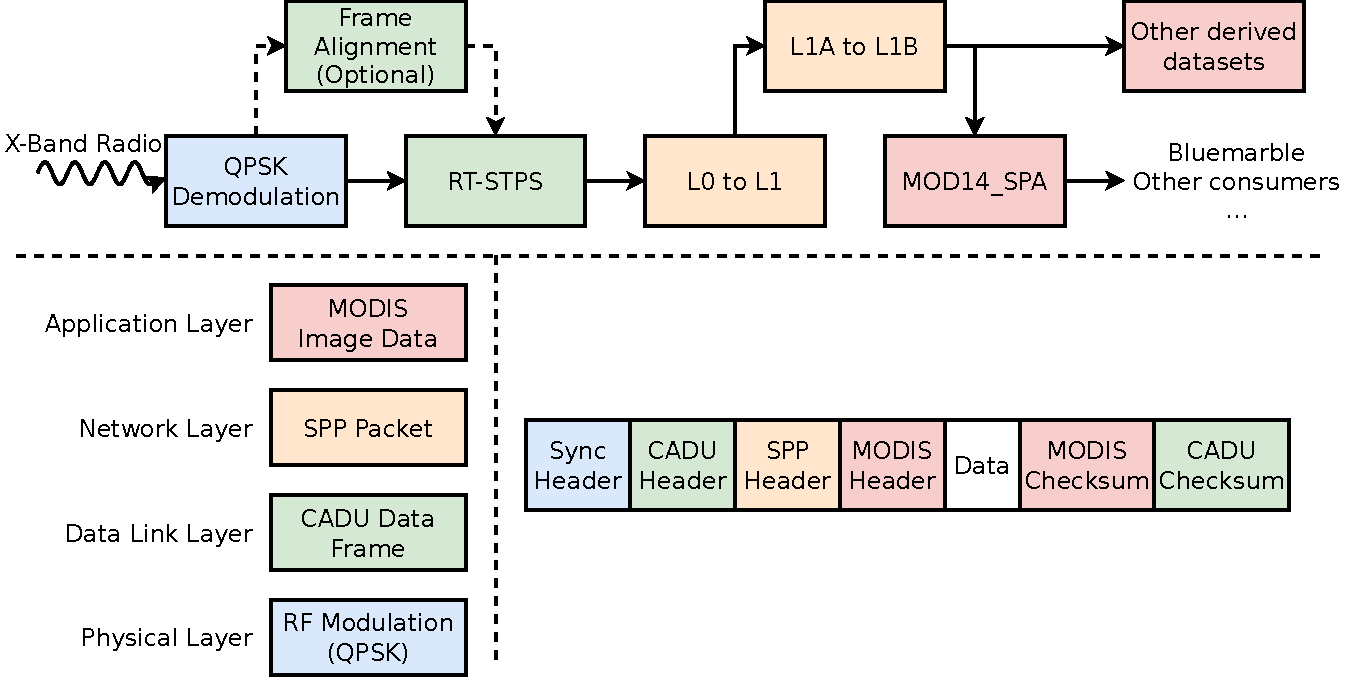
\includegraphics[width=\linewidth]{diagrams/attack_types.pdf}
    \caption{Illustration of the steps involved in processing MODIS image data and derived datasets, as well as the packet structure and layer within the network stack.}
    \label{fig:attack_types}
\end{figure}

% Through overshadowing the signal, an attacker can deliver arbitrary bytes to these processing stages, which were not designed with untrusted input data in mind.
% We demonstrate how the complex execution pathway includes input data being passed between several different processing applications unsafely.
% Ultimately, this results in the creation of a payload which gets inserted into the intermediate data structure, and may be triggered by a future reprocessing step.

% Part of the complexity of the system is due to its high number of dependencies, many of which come pre-bundled with the source code.
% These dependencies include outdated libraries with documented CVEs (Common Vulnerabilities and Exposures) which haven't been patched.
% For example, at the time of writing, MODISL1DB\_SPA comes bundled with HDF5 v1.12.0, which has 11 active CVEs.

% Interestingly, Too old for log4shell, for which it is not patched
% l0tol1 is distributed twice, there's no version control anywhere

% Reaching out over raw http to servers for data

\begin{comment}

\subsection{Attack description}

In each case, the attacker leverages different parts of the protocol to redirect the control flow of the program, either causing a denial of service, the leaking of sensitive data, or even arbitrary code execution.

Through the injection of standards-compliant frames, complete with synchronisation headers and checksums, the attacker can convince prior processing stages to decode and demultiplex an arbitrary byte sequence, delivering it as input to \textit{MODISL1DB\_SPA}.

The input to this algorithm is so-called \textit{Level 0} data, which is the body of a data frame with all communications artefacts, including synchronisation headers and checksums, removed.
Through the creation of a custom data frame, the attacker can encapsulate an arbitarary byte sequence which, when overshadowed over the existing signal, will result in the delivery of arbitrary bytes as the input to \textit{MODISL1DB\_SPA}.

We proceed to analyse several classes of attack made possible through this route, and enabled by insecure data handling practices.

\subsection{Exploiting downlink processing systems}

\subsubsection{Unprocessable malformed packets}

The software makes assumptions about the internal structure of the packets, which only hold for benign packets.
With the ability to inject arbitrary data, the attacker can craft packets to exploit oversights in the exception handling code for data parsing, and cause the program to crash.
Since the program processes packets in sets, a single malformed packet is sufficient to prevent the processing of the entire set.

Since the packet data is stored as a dataset for future processing, this attack also lets the attacker poison the dataset to make reprocessing of the entire set significantly harder.


\subsubsection{Latent arbitrary code execution}

In addition to near real-time data processing at the downlinks, past data is often reprocessed to take advantage of new processing alorithms, or to explore new results.
To support these use cases, the processing algorithms within MODISL1DB\_SPA are also available as command line tools, with adjustable configurations.

When run in SPA mode, the configuration used is always the same, which has resulted in a "golden path" through the execution of the program which is relatively secure.
However, by changing the initial configuration, a user could accidentally put the program into a mode which unsafely handles the input data.

Therefore, an attacker can poison the official datasets through the injection of packets, which cause no unsafe behaviour on first processing, but leverage vulnerabilities for arbitrary code execution when reprocessed under a different configuration.
These vulnerabilities have the potential to lie dormant in the official data sources as currently distributed by LAADS DAC, among other Direct Readout stations.

% TODO: go on to demonstrate the attack

\subsubsection{Reading unallocated memory}

Due to the design of the hardware on board the satellite, legitimate communications from the onboard instruments are guaranteed to hold to certain assumptions: for example, the packets are always of the same length, and the internal pointers between the packets are always aligned.

However, in this situation it becomes easy to let implicit assumptions about the structure of the data manifest themselves in the data processing.
Code for handling these exceptional cases is often less rigorously tested, because it generally doesn't occur in benign example cases.

However, by providing shorter packets than expected, with larger pointers than expected, we demonstrate how the attacker can take advantage of certain system components written in C to read off the end of the buffer into unallocated memory.
We demonstrate an execution pathway that would result in the resulting data being stored and uploaded to the public data archives, theoretically allowing the attacker to leak sensitive information from other processes within the memory of the computer.


\subsubsection{Exploiting bundled dependencies}

In order to make software distribution easier, and to create easily deployable systems that mostly "just work" when extracted into a certain location, the IPOPP algorithms generally come with many bundled dependencies in the source archive.
These files are compiled programs and libraries for the handling of input data, that are intended to work on specific architectures.

However, the practice of bundling libraries with software has long been considered bad from a security perspective, especially since the widespread use of package managers to resolve and install dependencies.
Doing so permits a similar ease of installation, but allows each library and program to be traced back to its dependency, independently updated, and uninstalled when no longer required.

Without a system for managing these dependencies, the system becomes incredibly brittle and hard to change; therefore, there are many dependencies currently present and depended upon that haven't been updated in nearly a decade.
Several of these dependencies have patchable security vulnerabilities for arbitrary code execution, that an attacker could take advantage of.

There are also a large number of dependencies that aren't used for any purpose and are just left around for legacy reasons.
Besides potentially being a risk for privilege escalation, the sheer number of redundant dependencies muddies the water and makes it difficult to discern which depencies need updating as a matter of urgency.

\end{comment}
